
\documentclass[]{article}
\usepackage{lmodern}
\usepackage{amssymb,amsmath}
\usepackage{ifxetex,ifluatex}
\usepackage{fixltx2e} % provides \textsubscript
\ifnum 0\ifxetex 1\fi\ifluatex 1\fi=0 % if pdftex
  \usepackage[T1]{fontenc}
  \usepackage[utf8]{inputenc}
\else % if luatex or xelatex
  \ifxetex
    \usepackage{mathspec}
    \usepackage{xltxtra,xunicode}
  \else
    \usepackage{fontspec}
  \fi
  \defaultfontfeatures{Mapping=tex-text,Scale=MatchLowercase}
  \newcommand{\euro}{€}
\fi
% use upquote if available, for straight quotes in verbatim environments
\IfFileExists{upquote.sty}{\usepackage{upquote}}{}
% use microtype if available
\IfFileExists{microtype.sty}{%
\usepackage{microtype}
\UseMicrotypeSet[protrusion]{basicmath} % disable protrusion for tt fonts
}{}
\usepackage{longtable,booktabs}
\usepackage{graphicx}
\makeatletter
\def\maxwidth{\ifdim\Gin@nat@width>\linewidth\linewidth\else\Gin@nat@width\fi}
\def\maxheight{\ifdim\Gin@nat@height>\textheight\textheight\else\Gin@nat@height\fi}
\makeatother
% Scale images if necessary, so that they will not overflow the page
% margins by default, and it is still possible to overwrite the defaults
% using explicit options in \includegraphics[width, height, ...]{}
\setkeys{Gin}{width=\maxwidth,height=\maxheight,keepaspectratio}
\ifxetex
  \usepackage[setpagesize=false, % page size defined by xetex
              unicode=false, % unicode breaks when used with xetex
              xetex]{hyperref}
\else
  \usepackage[unicode=true]{hyperref}
\fi
\hypersetup{breaklinks=true,
            bookmarks=true,
            pdfauthor={},
            pdftitle={},
            colorlinks=true,
            citecolor=blue,
            urlcolor=blue,
            linkcolor=magenta,
            pdfborder={0 0 0}}
\urlstyle{same}  % don't use monospace font for urls
\setlength{\parindent}{0pt}
\setlength{\parskip}{6pt plus 2pt minus 1pt}
\setlength{\emergencystretch}{3em}  % prevent overfull lines
\setcounter{secnumdepth}{0}

% Change margin size
\usepackage[margin=1in]{geometry}   

\usepackage{graphicx}
\usepackage{caption}
\usepackage{subcaption}

\date{}

\begin{document}

\section{Stats 242 Project}\label{stats-242-project}

\subsection{Medium data EDA visualization
benchmarks}\label{medium-data-eda-visualization-benchmarks}

8 June 2015

Zhewen Hu and Clark Fitzgerald

\subsubsection{Abstract}\label{abstract}

Which plotting libraries are fastest and most efficient for exploratory
analysis of medium sized data sets? In this report we compare several
popular plotting libraries by performing basic exploratory data analysis
(EDA) on a subset of the NYC taxi data set. Additionally we plot
informative maps about pickup and dropoff locations.

\subsubsection{Data}\label{data}

The data consists of a sample of the 2013 NYC taxi data from Assignment
5. These are available at http://www.andresmh.com/nyctaxitrips/ and
there is a description of the fields at
http://publish.illinois.edu/dbwork/open-data/. Since we are interested
in the performance of the libraries for working on data in memory we
wrote a program to randomly sample approximately 200 MB of the original
50 GB of data. This produced a CSV file containing 1.25 million rows and
21 columns. Below is an example:

\begin{longtable}[c]{@{}llll@{}}
\toprule
trip\_time\_in\_secs & pickup\_longitude & total\_amount &
\ldots{}\tabularnewline
\midrule
\endhead
1685 & -73.862839 & 38.3 &\tabularnewline
\ldots{} & & &\tabularnewline
\bottomrule
\end{longtable}

\subsubsection{Libraries}\label{libraries}

We compared the following open source libraries from R and Python:

\begin{enumerate}
\def\labelenumi{\arabic{enumi}.}
\itemsep1pt\parskip0pt\parsep0pt
\item
  \textbf{R} - Base R, using no extra packages
\item
  \textbf{ggplot2} - popular R library
\item
  \textbf{Matplotlib} - Established Python plotting library
\end{enumerate}

\subsection{Evaluation}\label{evaluation}

\subsubsection{Speed}\label{speed}

Speed was the primary focus. How long to make a single plot?

In general we saw Matplotlib was fastest with R not far behind. ggplot
was typically slower than R, but this is understandable because it's
putting more features on the plots.

\subsubsection{Aesthetics}\label{aesthetics}

Do the defaults look reasonable or are additional tweaks needed?

R does a nice job using clean, simple defaults. ggplot2 has the most
aesthetically pleasant defaults, but the font is a little small.
Matplotlib makes it easy to change the defaults through the use of style
sheets. A nitpick here is the need to always call \texttt{tight\_layout}
so that the labels are not cut off on the saved plot.

\subsubsection{Code Readability}\label{code-readability}

How expressive is the code? Extensibility? Maintainability? Learning
curve?

R and Matplotlib actually feel closer together than R and ggplot2.
ggplot2 uses Wilkinson's \emph{grammar of graphics} and requires data to
always be in a data frame. R's formula notation is handy for plots such
as the boxplot. Each library uses amount the same number of lines of
code to do the basic plots presented here.

\subsubsection{Reproducibility}\label{reproducibility}

We've taken care to make sure that this analysis can be reproduced. Our
principal tool for this is GNU make. pandoc makes for easy conversion
between formats. The scripts are written in such a way that they time
only the desired steps. This excludes the time required to load in the
data from disk. The timings were done serially on a 2010 Macbook with no
other programs running.

\begin{figure}[htbp]
\centering
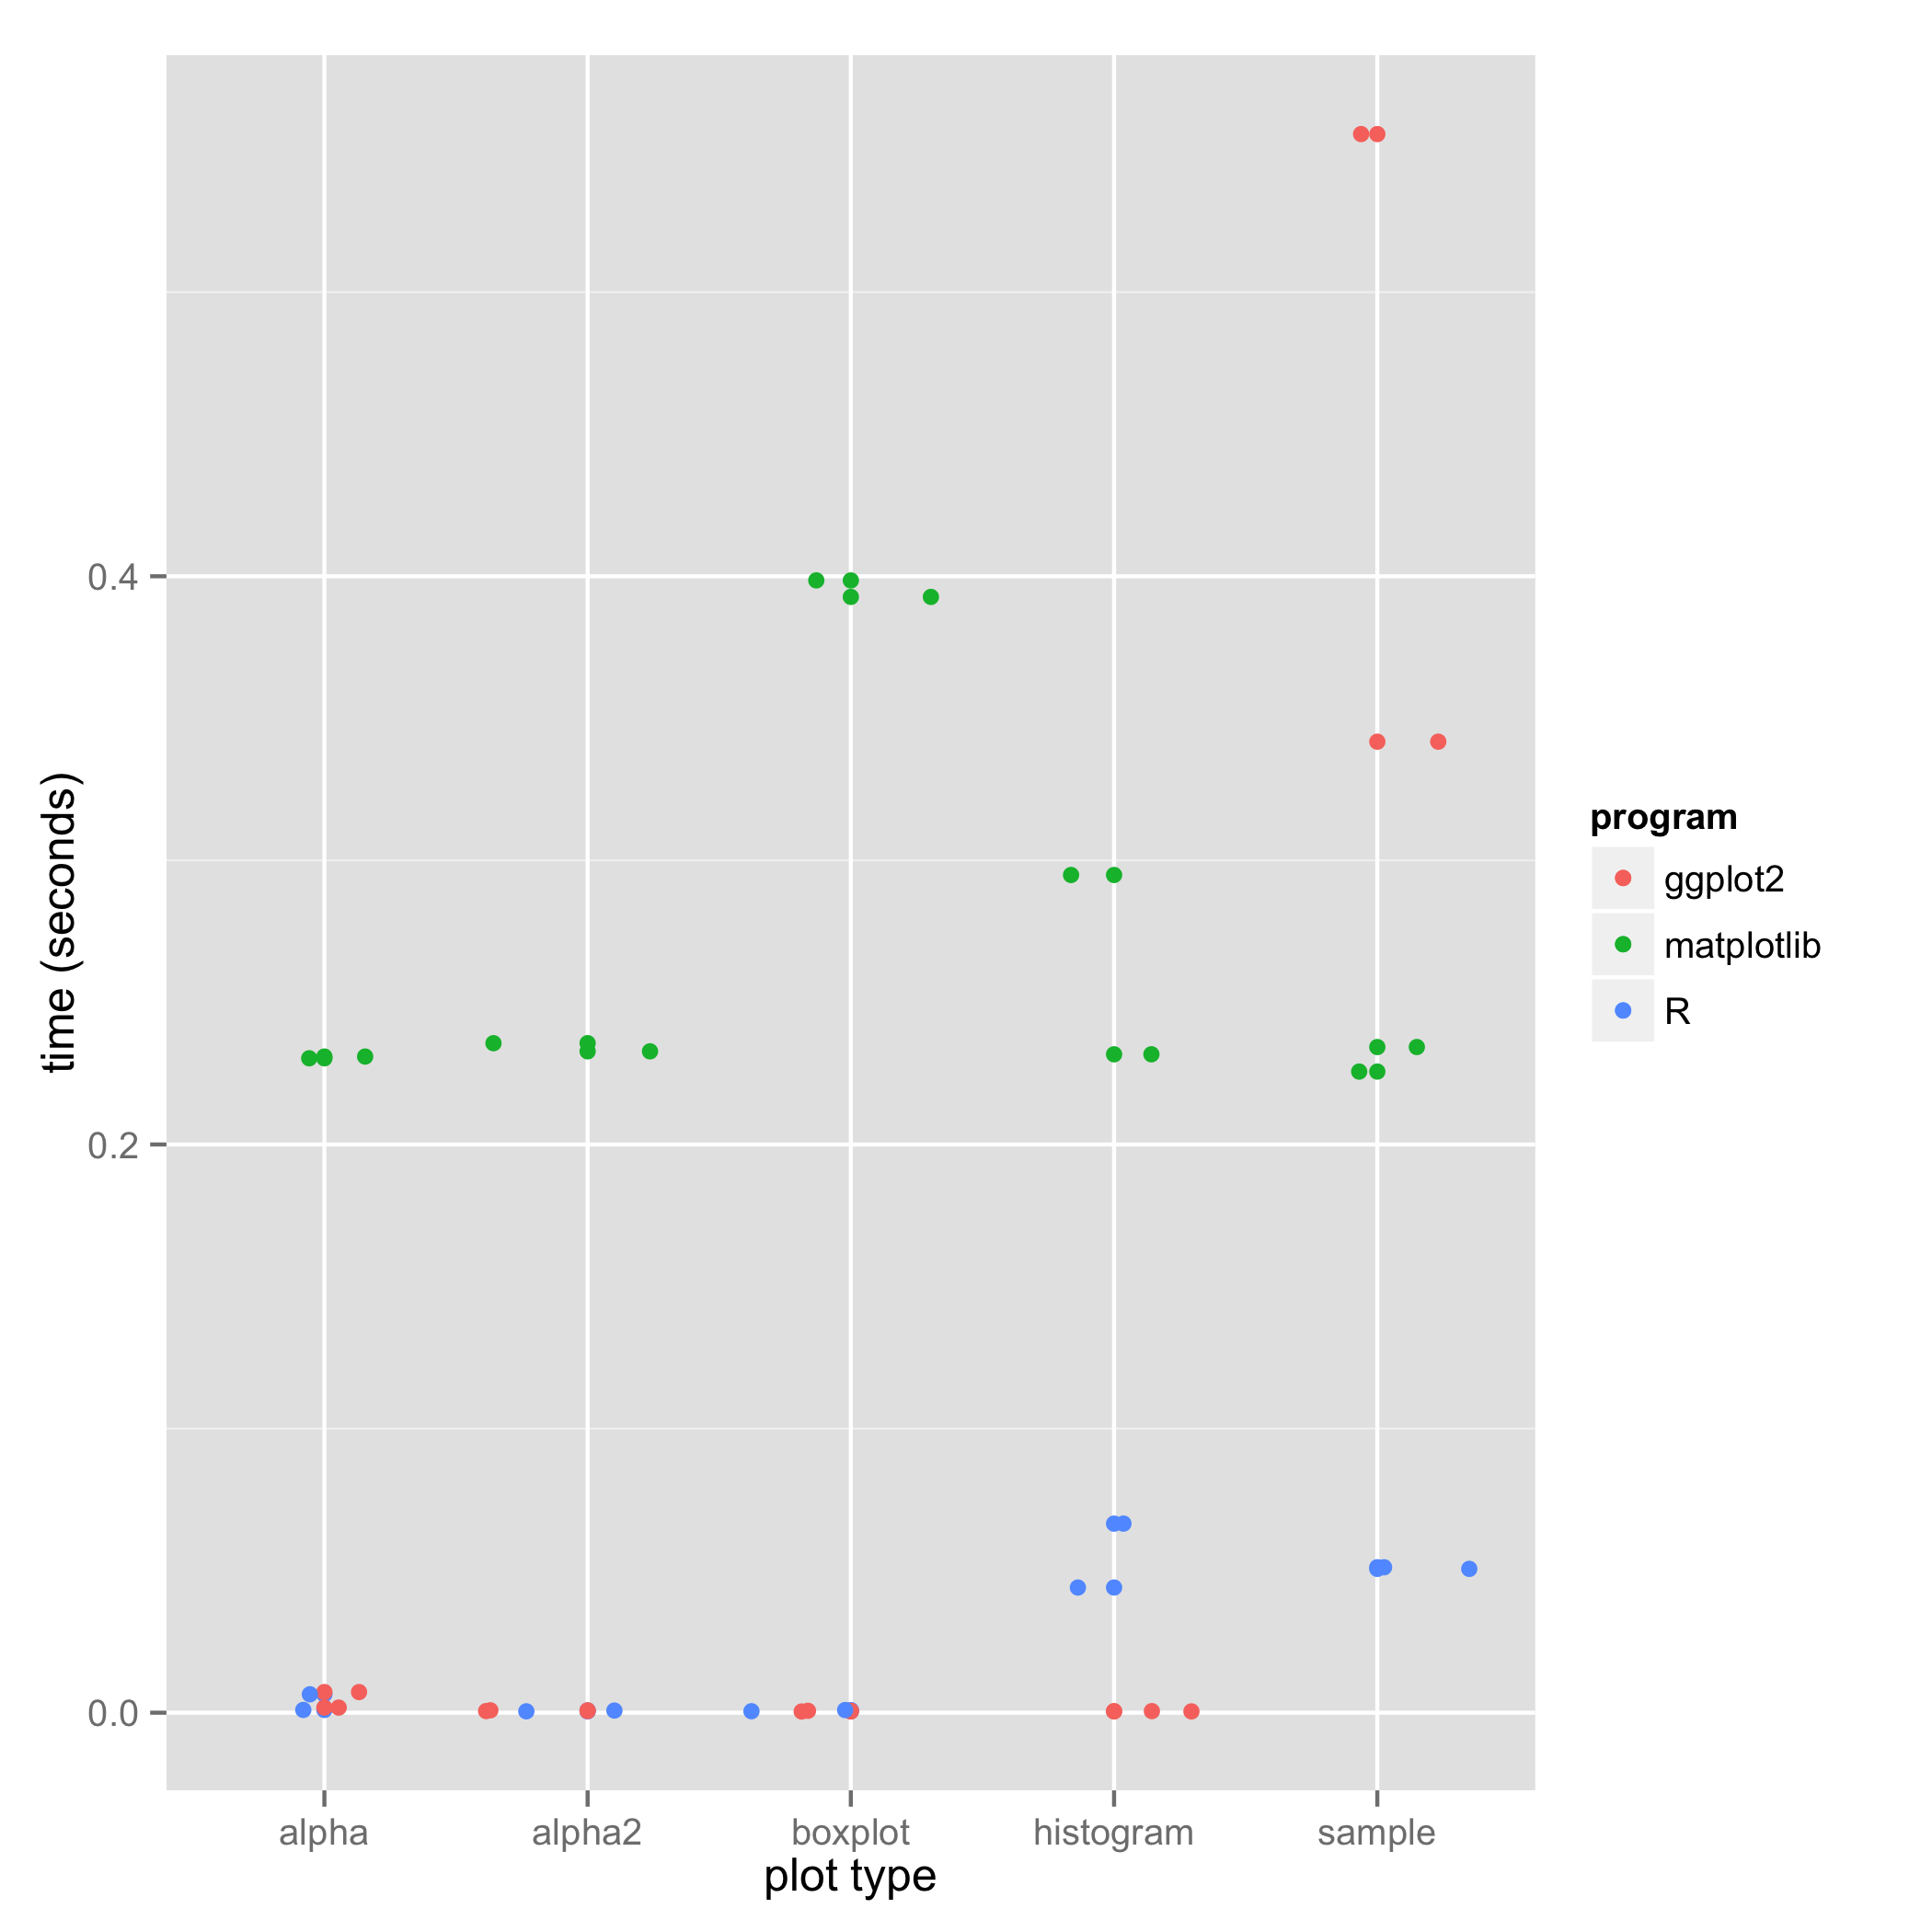
\includegraphics{timingplots.png}
\caption{The timings for each program}
\end{figure}

\begin{figure}[htbp]
\centering
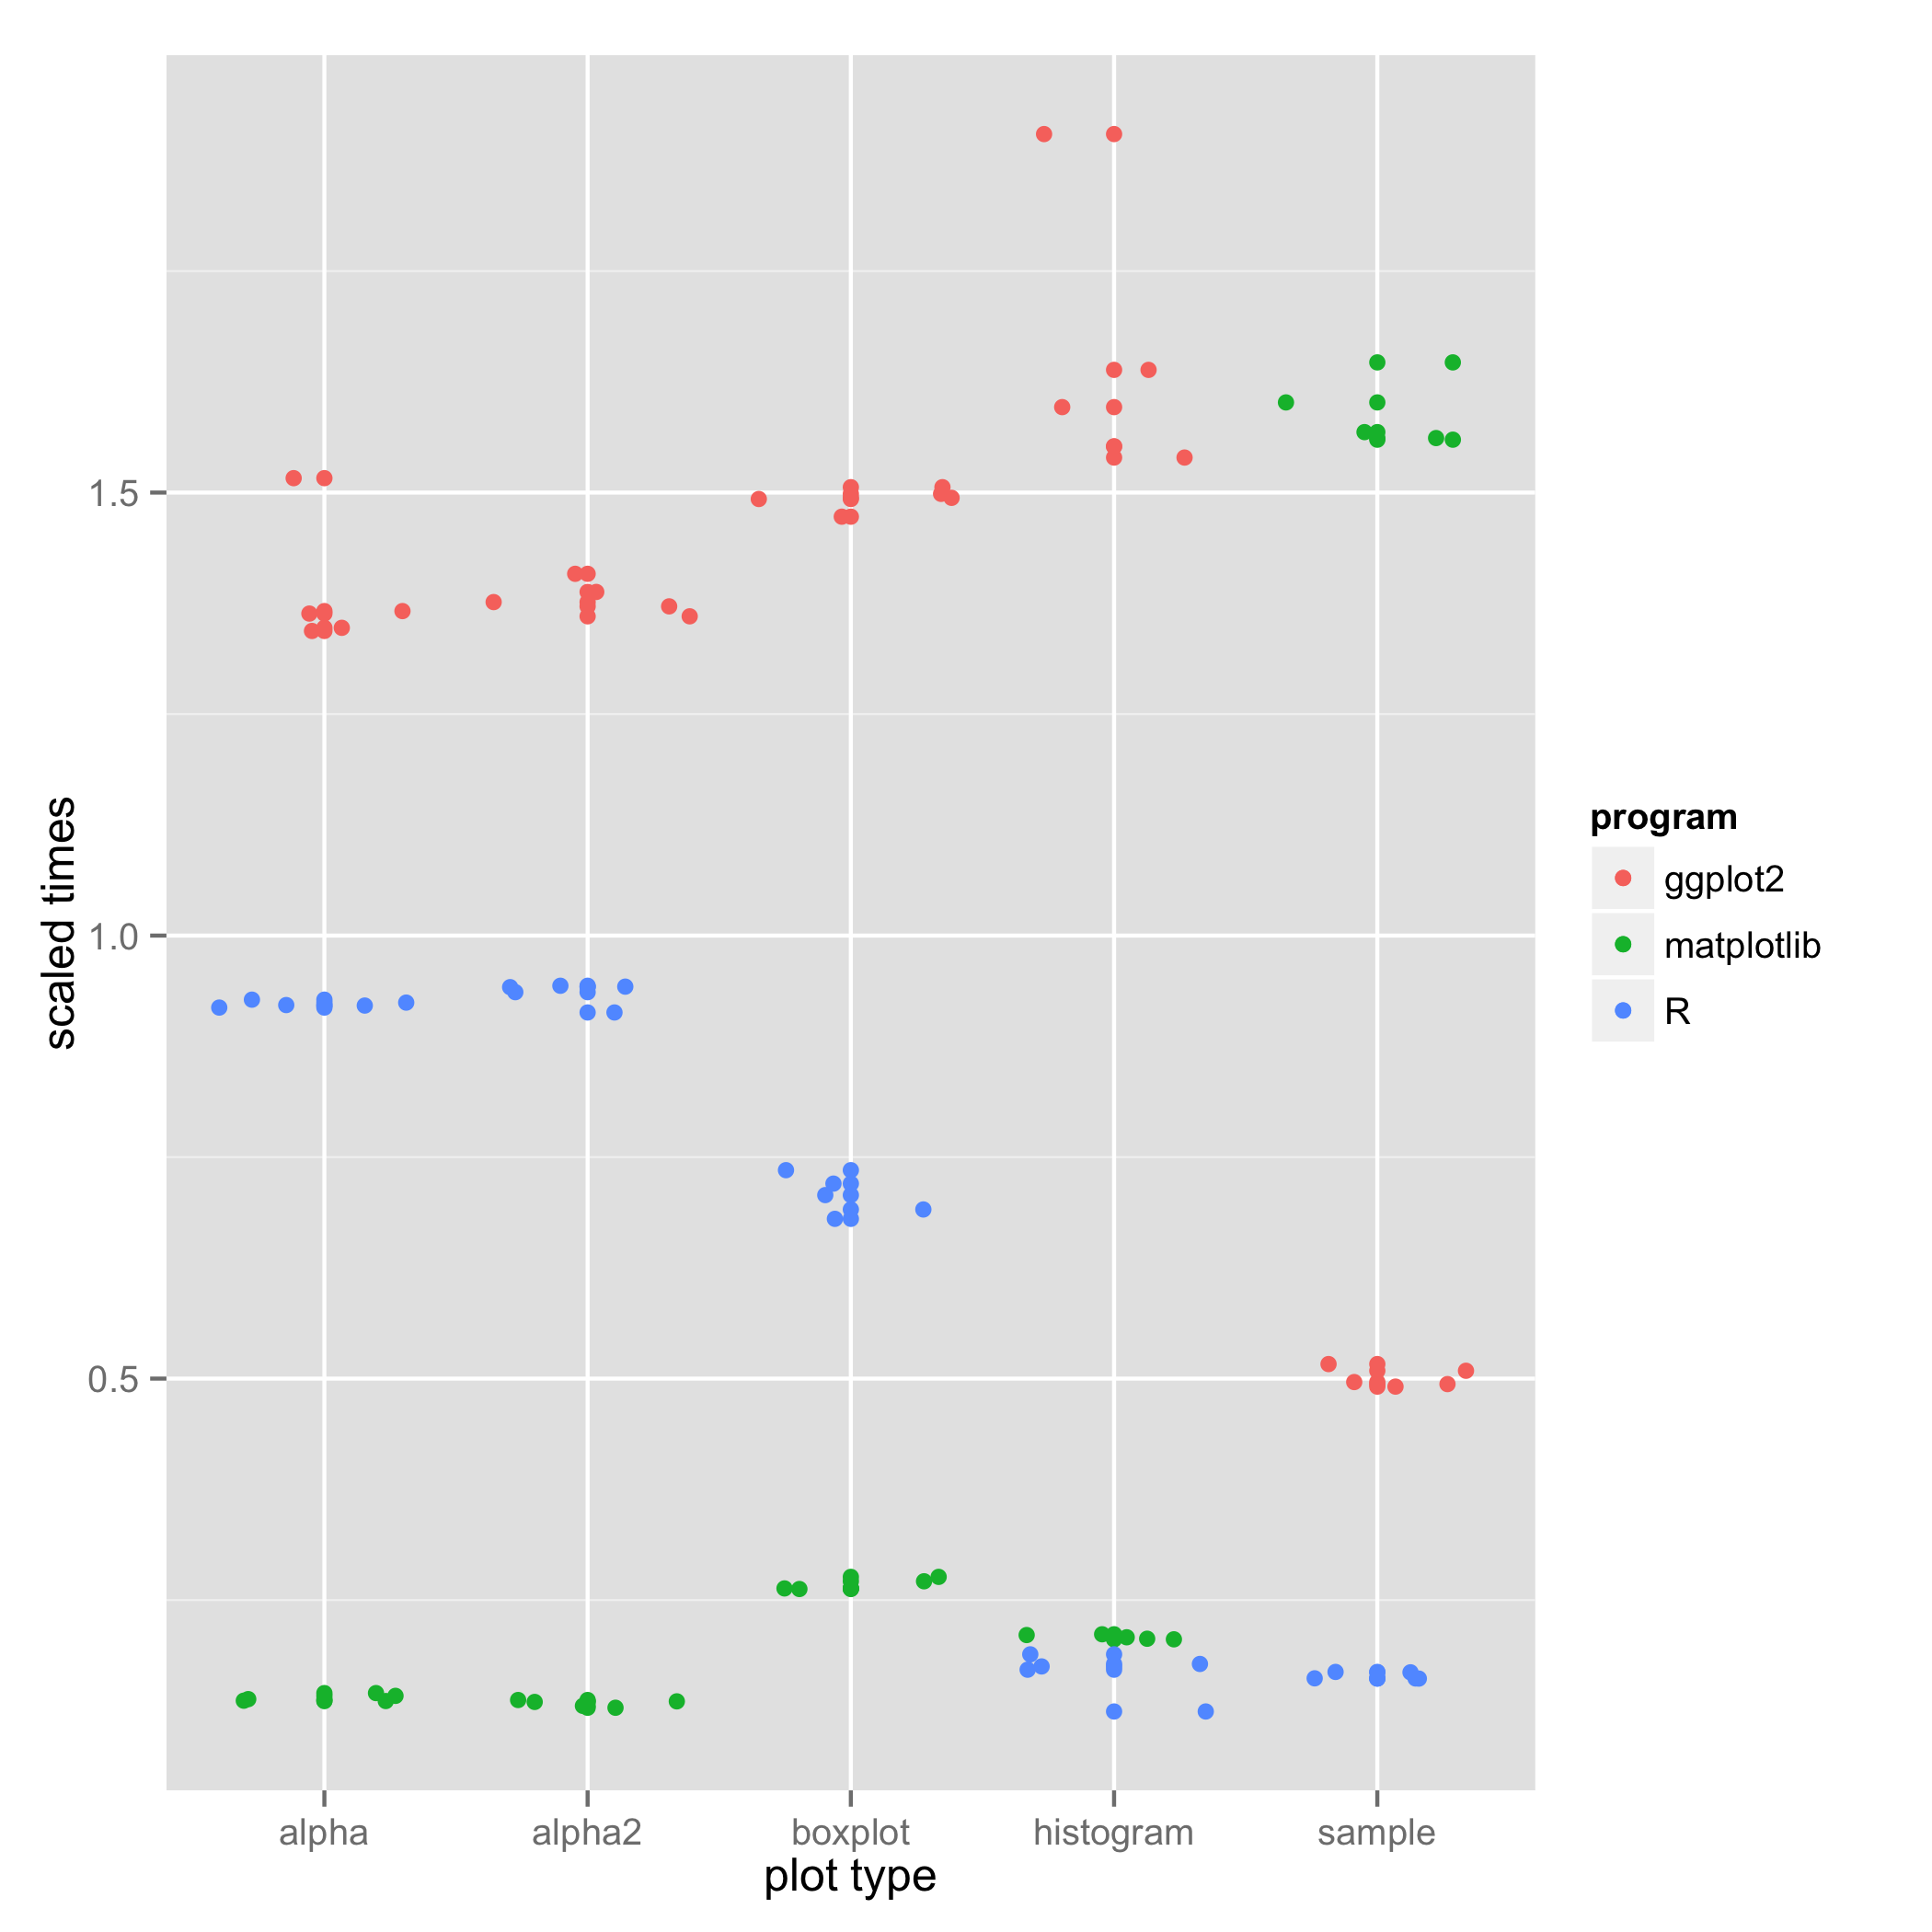
\includegraphics{timingplots2.png}
\caption{The timings for each program scaled within plot type}
\end{figure}

\section{Tasks}\label{tasks}

\subsubsection{Task 1: Histogram}\label{task-1-histogram}

Plot a histogram of the single variable \texttt{total\_amount} for
values of \texttt{total\_amount} less than 100.

In this plot we see the greatest difference in speed. R is fastest at
about 0.4 seconds. Matplotlib is right behind at 0.45 seconds. ggplot2
is significantly slower at about 3.5-4 seconds. These fast times makes
this a good choice of plot for EDA of large data sets.

Regarding aesthetics, R adds nice default labels.

\begin{figure}
        \centering
        \begin{subfigure}[b]{0.3\textwidth}
                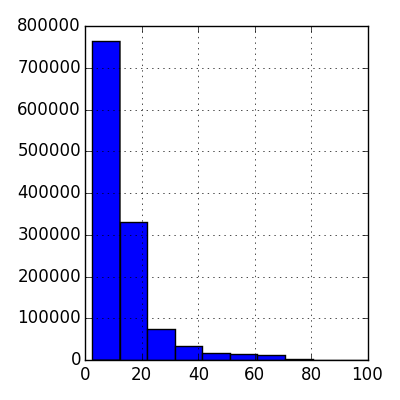
\includegraphics[width=\textwidth]{matplotlib/histogram.png}
                \caption{Matplotlib}
        \end{subfigure}%
        ~ %add desired spacing between images, e. g. ~, \quad, \qquad, \hfill etc.
          %(or a blank line to force the subfigure onto a new line)
        \begin{subfigure}[b]{0.3\textwidth}
                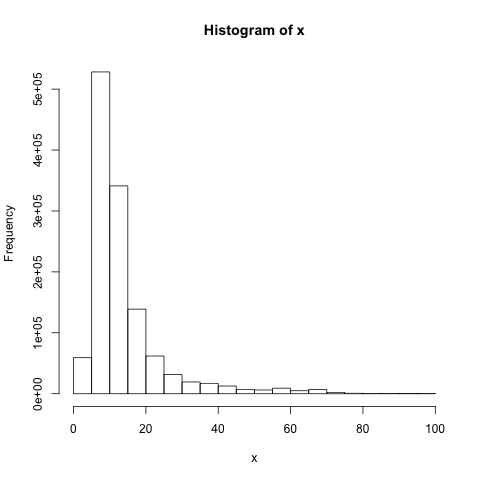
\includegraphics[width=\textwidth]{R/histogram.png}
                \caption{R}
        \end{subfigure}
        ~ %add desired spacing between images, e. g. ~, \quad, \qquad, \hfill etc.
          %(or a blank line to force the subfigure onto a new line)
        \begin{subfigure}[b]{0.3\textwidth}
                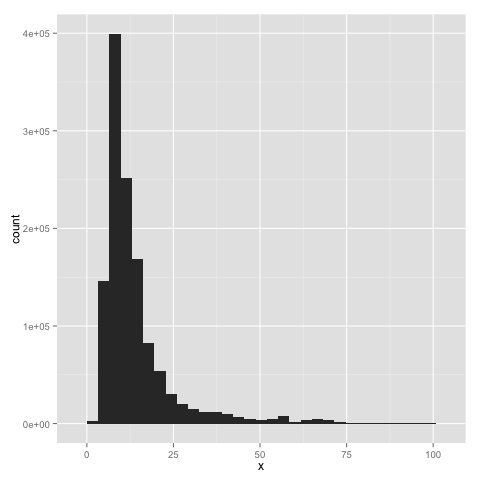
\includegraphics[width=\textwidth]{ggplot2/histogram.png}
                \caption{ggplot2}
        \end{subfigure}
        \caption{histograms}
\end{figure}

\subsubsection{Task 2: Alpha shading}\label{task-2-alpha-shading}

Scatter plot of two variables: trip time in minutes and
\texttt{total\_amount} where the points are semi transparent. This shows
the distribution of many points without completely overplotting. For
this timing we also convert \texttt{trip\_time\_in\_seconds} to minutes
by dividing by 60.

These plots revealed horizontal strata in the data where the total
amount corresponds to total fares between 50 and 70 dollars.

For these plots Matplotlib is much faster. It takes around 5 seconds to
plot 1 million alpha shaded points, while R took around 35 seconds and
ggplot was around 55 seconds.

Aesthetically R and ggplot2 make a nicer default choice of axis ranges,
since Matplotlib leaves an excessive amount of blank space.

\begin{figure}
        \centering
        \begin{subfigure}[b]{0.3\textwidth}
                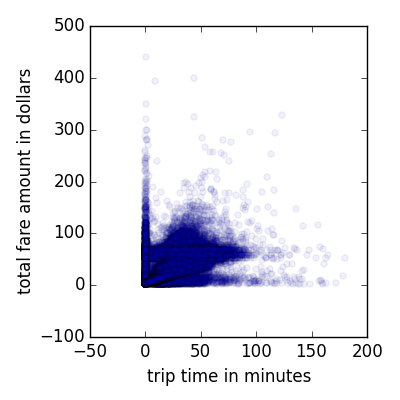
\includegraphics[width=\textwidth]{matplotlib/alpha.png}
                \caption{Matplotlib}
        \end{subfigure}%
        ~ %add desired spacing between images, e. g. ~, \quad, \qquad, \hfill etc.
          %(or a blank line to force the subfigure onto a new line)
        \begin{subfigure}[b]{0.3\textwidth}
                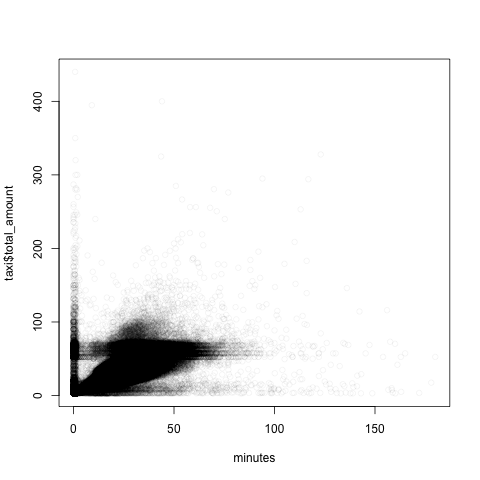
\includegraphics[width=\textwidth]{R/alpha.png}
                \caption{R}
        \end{subfigure}
        ~ %add desired spacing between images, e. g. ~, \quad, \qquad, \hfill etc.
          %(or a blank line to force the subfigure onto a new line)
        \begin{subfigure}[b]{0.3\textwidth}
                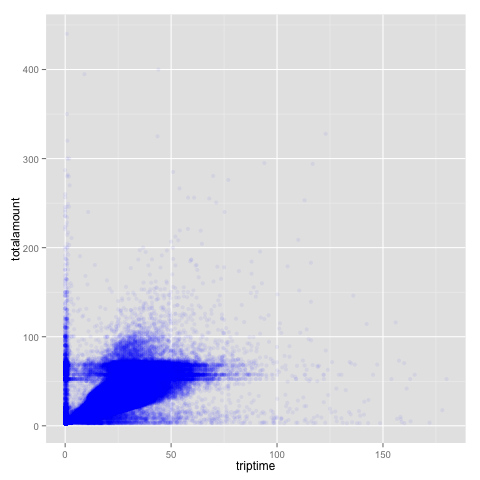
\includegraphics[width=\textwidth]{ggplot2/alpha.png}
                \caption{ggplot2}
        \end{subfigure}
        \caption{First alpha plot}
\end{figure}

We added an additional step to filter for rides less than 1 hour and
total amount less than 100.

\begin{figure}
        \centering
        \begin{subfigure}[b]{0.3\textwidth}
                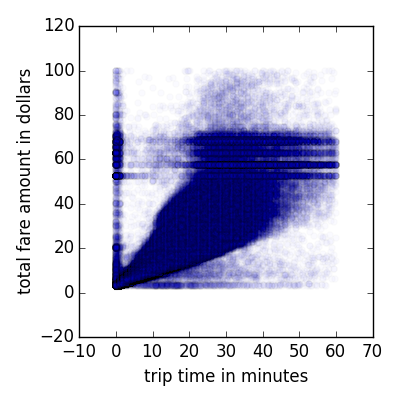
\includegraphics[width=\textwidth]{matplotlib/alpha2.png}
                \caption{Matplotlib}
        \end{subfigure}%
        ~ %add desired spacing between images, e. g. ~, \quad, \qquad, \hfill etc.
          %(or a blank line to force the subfigure onto a new line)
        \begin{subfigure}[b]{0.3\textwidth}
                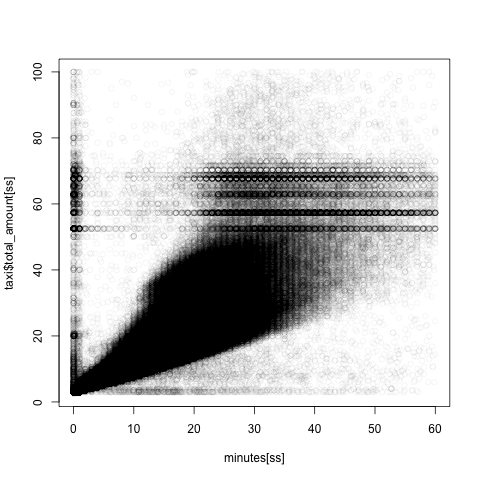
\includegraphics[width=\textwidth]{R/alpha2.png}
                \caption{R}
        \end{subfigure}
        ~ %add desired spacing between images, e. g. ~, \quad, \qquad, \hfill etc.
          %(or a blank line to force the subfigure onto a new line)
        \begin{subfigure}[b]{0.3\textwidth}
                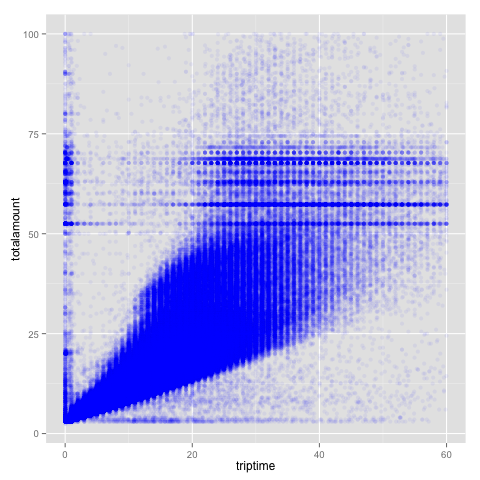
\includegraphics[width=\textwidth]{ggplot2/alpha2.png}
                \caption{ggplot2}
        \end{subfigure}
        \caption{Second alpha plot}
\end{figure}


\subsubsection{Task 3: Sampling}\label{task-3-sampling}

Perform the same scatter plot as the alpha shading, but instead of
plotting all points choose a random sample without replacement of 200
points.

This is one of the most informative plots. It demonstrates the increase
in total fare as the ride gets longer. It's also one of the
computationally cheapest plots. Matplotlib is much slower. We speculate
that this is because there is less overhead to create and save a single
plot in R.

We feel Matplotlib has nice defaults here regarding choice of scale and
visibility of points.

\begin{figure}
        \centering
        \begin{subfigure}[b]{0.3\textwidth}
                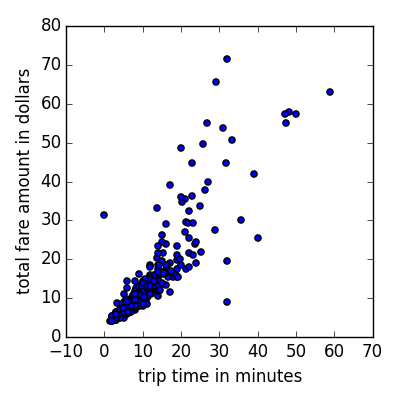
\includegraphics[width=\textwidth]{matplotlib/sample.png}
                \caption{Matplotlib}
        \end{subfigure}%
        ~ %add desired spacing between images, e. g. ~, \quad, \qquad, \hfill etc.
          %(or a blank line to force the subfigure onto a new line)
        \begin{subfigure}[b]{0.3\textwidth}
                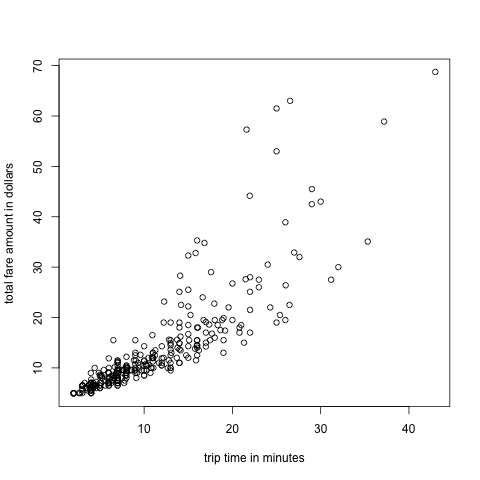
\includegraphics[width=\textwidth]{R/sample.png}
                \caption{R}
        \end{subfigure}
        ~ %add desired spacing between images, e. g. ~, \quad, \qquad, \hfill etc.
          %(or a blank line to force the subfigure onto a new line)
        \begin{subfigure}[b]{0.3\textwidth}
                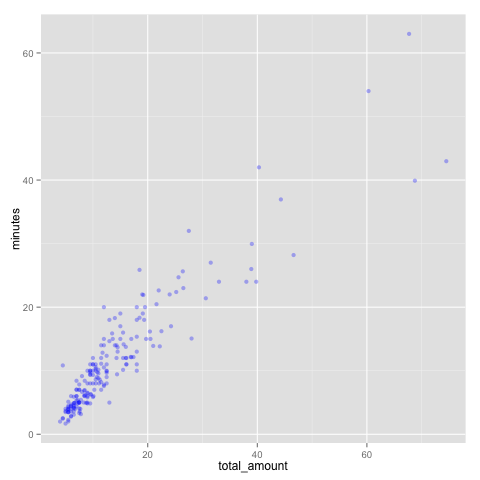
\includegraphics[width=\textwidth]{ggplot2/sample.png}
                \caption{ggplot2}
        \end{subfigure}
        \caption{samples}
\end{figure}

\subsubsection{Task 4: Boxplots}\label{task-4-boxplots}

Boxplots of \texttt{total\_amount} grouped by \texttt{payment\_type}
where \texttt{total\_amount} is less than 100. The long tails here
suggest that the distribution of the data is quite skewed.

Matplotlib was fastest here at 1.8 seconds. R was slower at 4.8 seconds
and ggplot2 was around 10.

Using the default pandas method in Matplotlib writes overlapping text
for the title, which is not good.

\begin{figure}
        \centering
        \begin{subfigure}[b]{0.3\textwidth}
                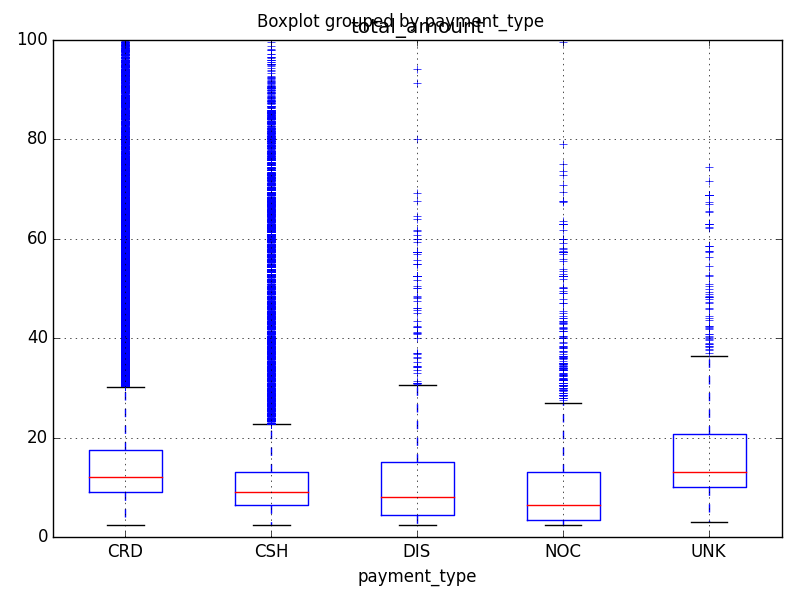
\includegraphics[width=\textwidth]{matplotlib/boxplot.png}
                \caption{Matplotlib}
        \end{subfigure}%
        ~ %add desired spacing between images, e. g. ~, \quad, \qquad, \hfill etc.
          %(or a blank line to force the subfigure onto a new line)
        \begin{subfigure}[b]{0.3\textwidth}
                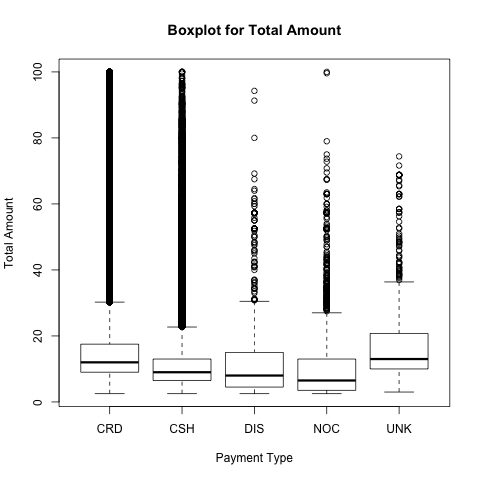
\includegraphics[width=\textwidth]{R/boxplot.png}
                \caption{R}
        \end{subfigure}
        ~ %add desired spacing between images, e. g. ~, \quad, \qquad, \hfill etc.
          %(or a blank line to force the subfigure onto a new line)
        \begin{subfigure}[b]{0.3\textwidth}
                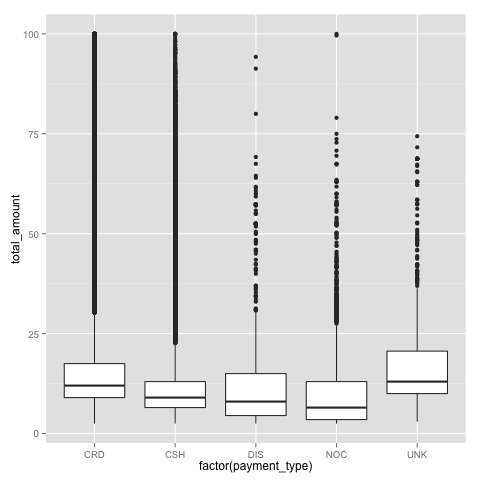
\includegraphics[width=\textwidth]{ggplot2/boxplot.png}
                \caption{ggplot2}
        \end{subfigure}
        \caption{boxplots}
\end{figure}

\subsection{Spatial Visualization}\label{spatial-visualization}

For this part, we test the performance of ggmap by visualizing the
pick-up longitude and latitude and drop-off latitude. The task is to see
that if ggmap works well in expressing data information.

If we get the map source from Google, it is not easy to adjust the range
of the map. Because Gmap source has its own default for the map. So it
is more flexible to source from stamen map library. We can see ggmap
does a good job in visualing the data points on the map. Also, it is
clear to see that taxi service is busier in Manhattan area than
Brooklyn. (The map plots are at the end of the report.)

\begin{figure}[htbp]
\centering
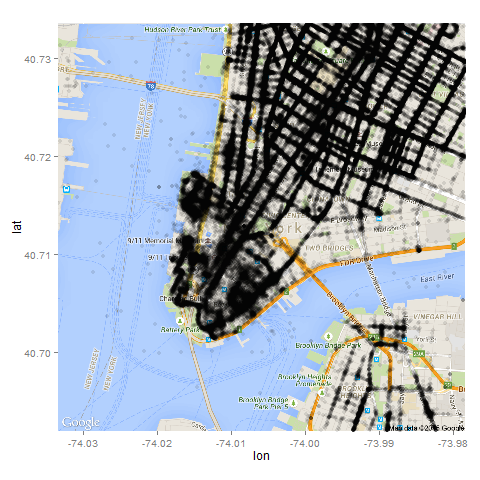
\includegraphics{R/pickup.png}
\caption{Source is Google Maps}
\end{figure}

\begin{figure}[htbp]
\centering
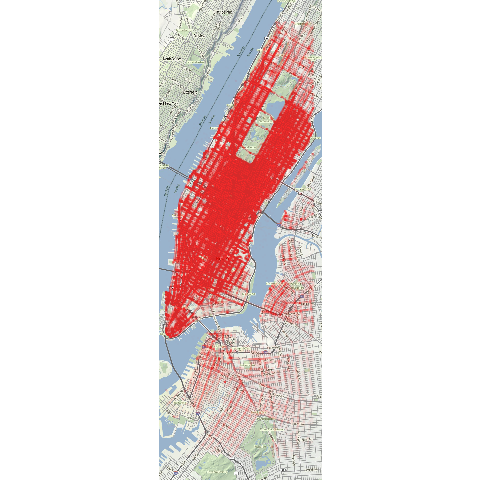
\includegraphics{R/dropoff.png}
\caption{Source is stamen map library}
\end{figure}

\subsection{Conclusion}\label{conclusion}

All programs tested are fully capable of doing exploratory data analysis
of millions of data points on a local laptop. Matplotlib is generally
faster, but not always. ggplot2 is slower than R, but has more beautiful
defaults and allows rapid creation of more complicated data analysis
graphics. R is quick to learn and provides nice defaults. ggmap works
pretty good in visualizing data. But do make sure the longitude and
latitude data is correct.

\end{document}
